\documentclass[11pt,a4paper,openany]{book}
\usepackage[margin=24mm]{geometry}
\usepackage{fontspec}
\IfFontExistsTF{Noto Serif}{\setmainfont{Noto Serif}}{\setmainfont{DejaVu Serif}}
\usepackage{amsmath,amssymb,tikz,enumitem,microtype}
\usepackage[hidelinks]{hyperref}
\setlength{\parindent}{0pt}
\setlength{\parskip}{6pt}
\setlist[enumerate]{leftmargin=*,itemsep=8pt}
\setlength{\emergencystretch}{2em}

\renewcommand{\contentsname}{Contents}
\begin{document}
\title{V-TALENT 2045\\ PHY101-A --- Units, scaling and algebra for physics\\\large Level 1 \textbar{} Mathematics for Physics}
\author{Dr. Dang Minh Tuan -- TS. Đặng Minh Tuấn}
\date{2026 \textbar{} Draft v1.0}
\maketitle
\tableofcontents
\chapter*{How to study}
Grades 8–9. Learn to turn measurements and physical statements into equations. No calculus is required. Prerequisites: fractions, powers of ten and basic equations.

Read the objective and answer the diagnostic before theory. Reproduce the worked solutions without looking, solve the exercises independently, then use the full solutions at the end to diagnose errors. Use a separate notebook for predictions, diagrams and checks. Original teaching text and exercises; external sources are reading locators, not reproduced. Draft pending independent review.
\chapter{Measurement, SI and dimensional reasoning}
\section{Objectives and diagnostic}
Convert compound units; derive units; distinguish an equation's dimensional consistency from its physical truth.

\textbf{Predict:} Why does 1 cm\textsuperscript{2} equal 0.0001 m\textsuperscript{2} rather than 0.01 m\textsuperscript{2}? Can a dimensionally correct formula still be false?
\section{Theory and derivations}
A measurement reports a number multiplied by a unit. Changing the unit changes the number, not the physical quantity. The SI base units used most often here are metre (m), kilogram (kg), second (s), ampere (A), kelvin (K) and mole (mol); the seventh is candela (cd). A centimetre is $10^{-2}$ m, a millimetre is $10^{-3}$ m and a micrometre is $10^{-6}$ m. Raising a length to a power also raises its conversion factor: $(1\,\mathrm{cm})^2=10^{-4}\,\mathrm{m^2}$ and $(1\,\mathrm{cm})^3=10^{-6}\,\mathrm{m^3}$.

Dimensions describe the kind of quantity: length $L$, mass $M$, time $T$. Speed has dimension $LT^{-1}$, acceleration $LT^{-2}$, force $MLT^{-2}$, pressure $ML^{-1}T^{-2}$ and energy $ML^2T^{-2}$. For example $p=F/A$ implies $\mathrm{Pa=N/m^2}$; $W=Fs$ (parallel constant force) gives $\mathrm{J=N\,m}$. Force and energy are not interchangeable even when numerical values coincide.

Both sides of a physical equation must have the same dimension; quantities added or subtracted must also agree dimensionally. Thus $s=vt+at^2$ passes a dimensional check, but it is not the correct constant-acceleration displacement formula when $v$ is the initial velocity: the second term needs the factor $1/2$. Dimensional analysis cannot determine dimensionless coefficients or prove a physical law. It can expose errors, narrow possible models and guide measurement.

Use conversion factors equal to one, such as $1000\,\mathrm{m}/1\,\mathrm{km}$ and $1\,\mathrm{h}/3600\,\mathrm{s}$. Multiply until unwanted units cancel. For density $\rho=m/V$, both mass and volume must be converted. Write the unit on every intermediate value. Keep unrounded values during calculation and round the final result according to the quality of the data.
\begin{center}
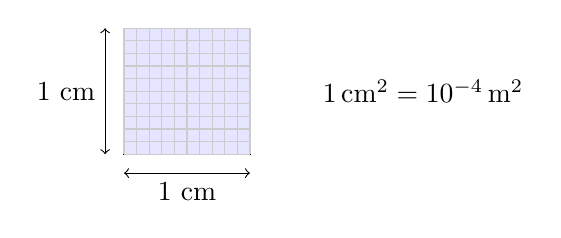
\begin{tikzpicture}[scale=.8]\draw[fill=blue!10] (0,0) rectangle (2,2);\draw[<->] (0,-.3)--node[below]{1 cm}(2,-.3);\draw[<->] (-.3,0)--node[left]{1 cm}(-.3,2);\draw[step=.2,gray!40] (0,0) grid (2,2);\node[right] at (3,1){$1\,\mathrm{cm^2}=10^{-4}\,\mathrm{m^2}$};\end{tikzpicture}
\end{center}
\section{Worked examples}
\subsection*{Example 1.1}
Convert 54 km/h and 1.25 g/cm\textsuperscript{3} into SI units.

\textbf{Solution.} $54(1000/3600)=15$ m/s. Also $1.25(10^{-3})/(10^{-6})=1250$ kg/m$^3$. The factor for volume is cubic.
\subsection*{Example 1.2}
A force of 120 N acts normally over 30 cm\textsuperscript{2}. Find pressure in Pa; explain why dividing by 30 gives the wrong SI value.

\textbf{Solution.} $A=30\times10^{-4}=0.003$ m$^2$. Then $p=120/0.003=40000$ Pa. The unconverted quotient 4 has unit N/cm$^2$, not Pa.
\subsection*{Example 1.3}
Which candidate could represent a time: v/g, g/v, or v\textsuperscript{2}/g? Here v is speed and g acceleration.

\textbf{Solution.} $[v/g]=(LT^{-1})/(LT^{-2})=T$. The second is $T^{-1}$; the third is $L$. Only $v/g$ has time dimension, though its coefficient and physical validity still need a model.
\section{Investigation}
Measure the sides and mass of a rectangular object three times. Calculate volume and density using SI and using g/cm\textsuperscript{3}, then convert and compare. Report the ruler resolution and explain why repeated readings do not remove a zero offset.
\section{Modern application and transfer}
A MEMS pressure sensor sees a pressure difference of 2500 Pa over a diaphragm area of 4 mm$^2$. The net pressure force in a uniform-pressure approximation is $F=pA=2500(4\times10^{-6})=0.010$ N. This shows why microfabricated sensors require careful unit conversion and force sensitivity. Transfer: if the same pressure acts on a diaphragm twice as wide with similar shape, predict the force; distinguish the force from the electrical signal, which requires a separate calibration model.
\section{Source-guided reading}
SW-14: ch. 14, §§14.3–14.4, pp. 304–306; JP-1.1: p. 3; JP-1.2: p. 4 (check ratio direction); JP-1.5: p. 8 (extension).
\section{Independent practice}
\begin{enumerate}
\item \textbf{PHY101-A-1.1}. Convert 7.2 km/h to m/s and 0.35 m\textsuperscript{2} to cm\textsuperscript{2}.
\item \textbf{PHY101-A-1.2}. A cube has side 4 cm and mass 172.8 g. Find density in kg/m\textsuperscript{3}.
\item \textbf{PHY101-A-1.3}. A 48 N load rests on four equal pads, each 2 cm\textsuperscript{2}. Find mean contact pressure.
\item \textbf{PHY101-A-1.4}. Given F=ma and P=Fv, derive the SI base unit of power.
\item \textbf{PHY101-A-1.5}. A proposed spring energy is kx where k has unit N/m. Test it and suggest a dimensionally consistent form using k and x.
\end{enumerate}
\chapter{Ratios, proportionality and scale}
\section{Objectives and diagnostic}
Distinguish direct, inverse and power laws; reason about area, volume and scaling.

\textbf{Predict:} If the radius of a sphere doubles, does its mass double? What must remain fixed?
\section{Theory and derivations}
For direct proportionality $y=kx$, the quotient $y/x$ is constant; the graph is a straight line through the origin. A straight line $y=kx+b$ with $b\ne0$ is not proportional. For inverse proportionality $y=k/x$, the product $xy$ is constant. In physics every proportionality statement is conditional: $p\propto1/A$ only if the normal force is fixed, and $I\propto V$ only for a constant resistance.

A power law $y=Cx^n$ implies $y_2/y_1=(x_2/x_1)^n$ when $C$ is fixed. Geometrically similar bodies with length factor $\lambda$ have area factor $\lambda^2$ and volume factor $\lambda^3$. If density is unchanged, mass scales as volume. For a body supported by a similar contact surface under its own weight, pressure scales as $\lambda^3/\lambda^2=\lambda$; a large model is not simply a small model with enlarged dimensions and unchanged stresses.

A useful derived quantity is the surface-to-volume ratio. For a cube of side $l$, $A/V=6/l$. For a sphere of radius $r$, $A/V=3/r$. Smaller objects offer more surface per unit volume. For heat exchange, chemical reaction or biological diffusion this ratio may matter, but actual rate also depends on material, temperature difference and boundary conditions. A scaling relation is an explanation of a trend, not a complete device model.
\begin{center}
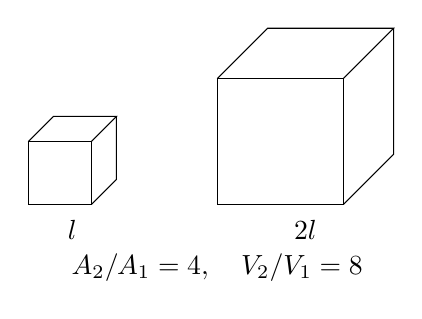
\begin{tikzpicture}[scale=.8]\draw (0,0) rectangle (1,1);\draw (0,1)--(.4,1.4)--(1.4,1.4)--(1,1);\draw (1,0)--(1.4,.4)--(1.4,1.4);\draw (3,0) rectangle (5,2);\draw (3,2)--(3.8,2.8)--(5.8,2.8)--(5,2);\draw (5,0)--(5.8,.8)--(5.8,2.8);\node at (.7,-.4){$l$};\node at (4.4,-.4){$2l$};\node at (3,-1){$A_2/A_1=4,\quad V_2/V_1=8$};\end{tikzpicture}
\end{center}
\section{Worked examples}
\subsection*{Example 2.1}
A resistor carries 0.20 A at 3 V. Predict current at 7.5 V if its resistance is unchanged.

\textbf{Solution.} $I_2/I_1=7.5/3=2.5$; $I_2=0.50$ A. Equivalently $R=15\,\Omega$. Heating may invalidate the assumption.
\subsection*{Example 2.2}
A model boat is enlarged by length factor 3 using the same density. How do mass, corresponding deck area and mean weight per deck area scale?

\textbf{Solution.} Mass factor $3^3=27$; area factor $3^2=9$; weight per area factor $27/9=3$. This is a geometric scaling estimate, not the actual local stress or buoyancy distribution.
\subsection*{Example 2.3}
A quantity obeys y=Cx\textsuperscript{2}. When x changes from 4 to 10, y changes from 12 to what value?

\textbf{Solution.} $y_2=12(10/4)^2=75$. Check $C=12/16=0.75$ and $0.75(100)=75$.
\section{Investigation}
Draw a table of cube side lengths 1, 2, 4 and 8 cm. Compute area, volume and A/V. Plot A/V against 1/l and explain the slope. Use SIM-M01 to compare your prediction.
\section{Modern application and transfer}
Divide a cube of side 12 mm into $4^3=64$ equal cubes of side 3 mm. If all surfaces become exposed, total area grows from $6(12)^2=864$ mm$^2$ to $64(6)(3)^2=3456$ mm$^2$, four times larger; total volume is unchanged. This is one reason particle size matters in materials processing and catalysis. Transfer: predict the area factor when the side is divided into $n$ parts, and explain why tightly packed particles do not expose all their surfaces.
\section{Source-guided reading}
JP-1.5: dimensional scaling, p. 8; SW-14: dimensional analysis, p. 305.
\section{Independent practice}
\begin{enumerate}
\item \textbf{PHY101-A-2.1}. An ideal spring stretches 8 mm under 2 N. Predict extension at 5 N within its linear range.
\item \textbf{PHY101-A-2.2}. A 60 N force acts over 0.020 m\textsuperscript{2}. Halve the area without changing force. Find both pressures.
\item \textbf{PHY101-A-2.3}. Similar solid spheres have radii 2 cm and 5 cm. Find mass and surface area ratios (large/small).
\item \textbf{PHY101-A-2.4}. At fixed speed the kinetic energy of an object doubles when mass doubles. At fixed mass what happens when speed triples?
\item \textbf{PHY101-A-2.5}. A sealed cubic package is scaled up by 2. If heat loss per unit surface area is identical and internal heat capacity is proportional to volume, compare the initial cooling rates.
\end{enumerate}
\chapter{Algebra as a physical modelling tool}
\section{Objectives and diagnostic}
Rearrange equations, solve systems, identify physically admissible roots and represent linear calibration.

\textbf{Predict:} A formula has two algebraic roots. Must both be physically possible?
\section{Theory and derivations}
A physical equation is a constraint among quantities, not just a recipe for substitution. Rearrange symbolically first so that dependence on inputs is visible. From $P=UI$ and $U=IR$, derive $P=I^2R=U^2/R$ for an ohmic resistor. The two expressions imply different trends depending on whether current or voltage is held fixed. Before dividing by a quantity, check that it is not zero.

Linear relations with offsets have form $y=ax+b$. For two distinct calibration inputs, $a=(y_2-y_1)/(x_2-x_1)$ and $b=y_1-ax_1$. The slope has units of output per input, the intercept has output units. Calibration inverts the relation: $x=(y-b)/a$ if $a\ne0$. Interpolation between tested points is usually more defensible than extrapolation. Two points always define a line, so further data are needed to test linearity.

Systems of equations arise when several conditions must hold simultaneously. In ideal heat mixing with equal specific heat and negligible loss, $m_h(T_h-T)=m_c(T-T_c)$; therefore $T=(m_hT_h+m_cT_c)/(m_h+m_c)$. It lies between the two initial temperatures for positive masses. In motion, $s=ut+at^2/2$ may have two roots; use initial time, direction, contact and the domain of the motion model to select the valid root. A solution is complete only when substituted back and physically interpreted.
\begin{center}
\begin{tikzpicture}[x=1.05cm,y=.7cm]\draw[->](0,0)--(5.3,0)node[right]{$x$};\draw[->](0,0)--(0,6)node[above]{$y$};\draw[thick,blue](0,1)--(4.5,5.5);\fill (1,2)circle(2pt) (4,5)circle(2pt);\draw[dashed](1,2)--(4,2)--(4,5);\node at (2.5,1.7){$\Delta x$};\node[right]at(4,3.5){$\Delta y$};\node[left]at(0,1){$b$};\end{tikzpicture}
\end{center}
\section{Worked examples}
\subsection*{Example 3.1}
A sensor reads 0.40 V at 0 N and 2.40 V at 10 N. Assuming linear response, estimate force at 1.60 V.

\textbf{Solution.} $a=(2.40-0.40)/10=0.20$ V/N; $U=0.40+0.20F$. Thus $F=(1.60-0.40)/0.20=6$ N. This lies inside the calibrated interval.
\subsection*{Example 3.2}
Mix 200 g of water at 65\textdegree{}C with 300 g at 15\textdegree{}C in an ideal insulated container. Find equilibrium temperature.

\textbf{Solution.} Equal specific heats cancel: $200(65-T)=300(T-15)$. Then $500T=17500$ and $T=35^\circ$C. The result is closer to the larger mass's temperature.
\subsection*{Example 3.3}
An object has x=3t\textsuperscript{2}-6t (m), t\ensuremath{\ge}0. When is it at x=9 m?

\textbf{Solution.} $3t^2-6t-9=0$ gives $(t-3)(t+1)=0$. The roots are 3 s and -1 s; discard -1 because the stated domain is $t\ge0$. Check $x(3)=9$ m.
\section{Investigation}
Use a spring and known small masses safely. Plot extension versus load; estimate slope from separated points, then check an intermediate point. If the spring does not return to its original length, stop: the elastic model is no longer reliable.
\section{Modern application and transfer}
For a battery-powered temperature logger, a linear sensor might produce 0.50 V at 0\textdegree{}C and 0.90 V at 40\textdegree{}C. The calibration slope is 0.010 V/\textdegree{}C; an output of 0.73 V means 23\textdegree{}C. Transfer: a zero-offset drift of +0.020 V would bias the estimate upward by 2\textdegree{}C if ignored. Explain how a reference thermometer can detect this drift and why real sensors need validation at more than two temperatures.
\section{Source-guided reading}
SJ-01: Functions, p. 9 (selected reading; calculus deferred); SW-14: graphs, pp. 305–306; JP-C7: linear fit, pp. 288–292 (teacher extension).
\section{Independent practice}
\begin{enumerate}
\item \textbf{PHY101-A-3.1}. A 12 V source supplies an ideal 6 \ensuremath{\Omega} resistor. Find current and power; then double resistance at fixed voltage.
\item \textbf{PHY101-A-3.2}. A force sensor reads 0.6 V at 2 N and 1.8 V at 8 N. Find its linear equation and estimate force at 1.2 V.
\item \textbf{PHY101-A-3.3}. How much 80\textdegree{}C water must be mixed with 150 g of 20\textdegree{}C water to reach 40\textdegree{}C, neglecting losses?
\item \textbf{PHY101-A-3.4}. Two objects have total mass 500 g and their masses differ by 80 g. Find both masses.
\item \textbf{PHY101-A-3.5}. An object moves according to x=2t\textsuperscript{2}+2t for t\ensuremath{\ge}0. Find when x=12 m.
\end{enumerate}
\chapter{Estimation, uncertainty and testing a model}
\section{Objectives and diagnostic}
Estimate orders of magnitude, distinguish measurement resolution from accuracy and compare predictions with observations.

\textbf{Predict:} If a calculator reports 3.14159265, does the experiment justify all those digits?
\section{Theory and derivations}
An order-of-magnitude estimate identifies a plausible scale before detailed calculation. Break an unknown into measurable or defensible factors. For example, a room volume can be estimated from length, width and height; multiply by an assumed air density to estimate air mass. Record assumptions and distinguish measured from estimated quantities. If a result changes greatly when an uncertain assumption changes slightly, that assumption needs better evidence.

Resolution is the smallest indicated increment of an instrument. Accuracy concerns closeness to a reference or true value; precision concerns agreement among repeated results. A repeated measurement may be precise yet inaccurate due to systematic bias. For a simple classroom bound, express each positive measurement as $x\pm\delta x$ and use minimum/maximum possible values. This bound is not automatically a standard deviation or confidence interval.

If $z=xy$ and both variables are positive, the extreme bounds are $(x-\delta x)(y-\delta y)$ and $(x+\delta x)(y+\delta y)$. For $z=x/y$ with $y-\delta y>0$, the minimum uses the smallest numerator and largest denominator; the maximum uses the reverse. Compare model predictions with measured bounds; a discrepancy may indicate model failure, unrecognised uncertainty or a measurement fault. Agreement is not proof that a model is uniquely correct.
\begin{center}
\begin{tikzpicture}[x=.8cm]\draw[->](0,0)--(8,0)node[right]{$x$};\draw[thick,blue](1,1)--(5,1);\draw(1,.8)--(1,1.2)(5,.8)--(5,1.2);\fill(3,1)circle(2pt);\node[above]at(3,1.3){$x\pm\delta x$};\draw[thick,dashed](4,0)--(4,2);\node[above]at(4,2){$x_{\rm model}$};\end{tikzpicture}
\end{center}
\section{Worked examples}
\subsection*{Example 4.1}
Estimate air mass in a 5 m \ensuremath{\times} 4 m \ensuremath{\times} 3 m room using density 1.2 kg/m\textsuperscript{3}.

\textbf{Solution.} $V=60$ m$^3$, $m=1.2(60)=72$ kg. This assumes uniform density and ignores furniture displacement; the estimate is of order $10^2$ kg.
\subsection*{Example 4.2}
A measured rectangle has sides 10.0\ensuremath{\pm}0.1 cm and 5.0\ensuremath{\pm}0.1 cm. Find the area and extreme bounds.

\textbf{Solution.} Central $A=50.0$ cm$^2$. Lower $9.9(4.9)=48.51$; upper $10.1(5.1)=51.51$ cm$^2$. The interval is slightly asymmetric; a conservative rounded bound is about $50.0\pm1.6$ cm$^2$.
\subsection*{Example 4.3}
A thermometer repeatedly gives 24.8\textdegree{}C in a reference bath at 25.0\textdegree{}C. Explain what repeated agreement establishes and what it does not.

\textbf{Solution.} The repeated readings indicate good repeatability at the displayed resolution. They differ from the reference by -0.2\textdegree{}C. A systematic offset is plausible, but reference uncertainty and other conditions must be checked; repeatability alone cannot establish accuracy.
\section{Investigation}
Estimate the volume of a classroom from paced distances, then measure with a tape. Compare the two estimates and list at least three uncertainty sources. Do not treat the tape result as exact.
\section{Modern application and transfer}
A solar-powered data logger uses 0.30 W for 24 h, or 7.2 Wh per day. If a small panel provides an average of 2 W during 4 effective sunlight hours, gross energy is 8 Wh. With 75 percent storage/conversion efficiency, usable energy is 6 Wh, insufficient by 1.2 Wh. Transfer: find minimum average panel power for those assumptions; explain why variable weather and battery ageing require reserve capacity.
\section{Source-guided reading}
SW-14: §§14.1–14.4, pp. 301–306; JP-C7: §§7.1–7.5, pp. 273–292.
\section{Independent practice}
\begin{enumerate}
\item \textbf{PHY101-A-4.1}. Estimate the mass of a 2 m \ensuremath{\times} 1 m \ensuremath{\times} 1 mm aluminium sheet using density 2700 kg/m\textsuperscript{3}.
\item \textbf{PHY101-A-4.2}. Distance is 20.0\ensuremath{\pm}0.2 m and time is 4.0\ensuremath{\pm}0.1 s. Find speed and extreme bounds.
\item \textbf{PHY101-A-4.3}. A ruler always adds 0.3 cm to a direct length reading. Ten readings average 12.4 cm. If the offset is known exactly, correct the mean.
\item \textbf{PHY101-A-4.4}. A model predicts 8.0 N; measured force is 7.4\ensuremath{\pm}0.2 N. Is the prediction inside the stated bound? What should be investigated?
\item \textbf{PHY101-A-4.5}. For the solar logger above, determine minimum panel average power during four effective sunlight hours at 75 percent efficiency.
\end{enumerate}
\chapter*{References and simulations}
Swiss Physics Olympiad Script, 3rd ed. (2019).\par
The Committee of Japan Physics Olympiad (2014). \textit{Physics Olympiad: Basic to Advanced Exercises}. World Scientific.\par
Tan Chien Hao (2024). \textit{Freshman Physics}.\par
\url{https://diavn.github.io/truongchuyen/physics-curriculum.html}\par
\url{https://diavn.github.io/truongchuyen/physics-math-lab.html}
\appendix
\chapter{Full solutions to independent practice}
\section{Measurement, SI and dimensional reasoning}
\begin{enumerate}
\item \textbf{PHY101-A-1.1}. $7.2/3.6=2$ m/s; $0.35\times10^4=3500$ cm$^2$.
\item \textbf{PHY101-A-1.2}. $V=64$ cm$^3$; $\rho=172.8/64=2.7$ g/cm$^3=2700$ kg/m$^3$.
\item \textbf{PHY101-A-1.3}. Total area $8\times10^{-4}$ m$^2$; $p=48/(8\times10^{-4})=60000$ Pa. Equal loading gives the same pressure on each pad.
\item \textbf{PHY101-A-1.4}. $[F]=MLT^{-2}$; multiply by $LT^{-1}$ to obtain $ML^2T^{-3}$, so W = kg m$^2$ s$^{-3}$.
\item \textbf{PHY101-A-1.5}. $kx$ has force units. $kx^2$ has energy units; the actual ideal spring law is $U=kx^2/2$ relative to the unstretched state, established from work rather than units alone.
\end{enumerate}
\section{Ratios, proportionality and scale}
\begin{enumerate}
\item \textbf{PHY101-A-2.1}. $x_2=8(5/2)=20$ mm.
\item \textbf{PHY101-A-2.2}. $p_1=60/0.020=3000$ Pa; $p_2=60/0.010=6000$ Pa.
\item \textbf{PHY101-A-2.3}. $\lambda=5/2$; mass ratio $(5/2)^3=125/8$; area ratio $(5/2)^2=25/4$.
\item \textbf{PHY101-A-2.4}. $K=mv^2/2$, so $K_2/K_1=3^2=9$.
\item \textbf{PHY101-A-2.5}. Heat loss power scales by 4; heat capacity by 8. Since $|dT/dt|$ is power divided by heat capacity, the initial cooling rate is half. At Level 1 interpret this as temperature decrease per short time interval.
\end{enumerate}
\section{Algebra as a physical modelling tool}
\begin{enumerate}
\item \textbf{PHY101-A-3.1}. $I=12/6=2$ A, $P=24$ W. With $R=12\,\Omega$, $I=1$ A, $P=12$ W.
\item \textbf{PHY101-A-3.2}. $a=(1.8-0.6)/6=0.2$ V/N; $b=0.6-0.2(2)=0.2$ V. $F=(1.2-0.2)/0.2=5$ N.
\item \textbf{PHY101-A-3.3}. $m(80-40)=150(40-20)$, so $40m=3000$ and $m=75$ g.
\item \textbf{PHY101-A-3.4}. $m_1+m_2=500$, $m_1-m_2=80$. Add: $2m_1=580$; $m_1=290$ g, $m_2=210$ g.
\item \textbf{PHY101-A-3.5}. $t^2+t-6=(t+3)(t-2)=0$. Accept 2 s, reject -3 s.
\end{enumerate}
\section{Estimation, uncertainty and testing a model}
\begin{enumerate}
\item \textbf{PHY101-A-4.1}. $V=2(1)(0.001)=0.002$ m$^3$; $m=5.4$ kg.
\item \textbf{PHY101-A-4.2}. Central 5.0 m/s; lower $19.8/4.1\approx4.83$; upper $20.2/3.9\approx5.18$ m/s.
\item \textbf{PHY101-A-4.3}. $12.4-0.3=12.1$ cm. Averaging did not remove the offset; other uncertainties remain.
\item \textbf{PHY101-A-4.4}. Bound 7.2–7.6 N excludes 8.0 N. Check calibration, omitted forces and whether the model prediction itself has uncertainty; do not immediately declare the law false.
\item \textbf{PHY101-A-4.5}. $0.75P(4)=7.2$ Wh, so $P=2.4$ W. This just balances the model's daily energy; it provides no reserve.
\end{enumerate}
\end{document}
